\begin{frame}{$d(K^-, n)$ reaction and J-PARC E31}
  \begin{tabular}{cc}
    \begin{minipage}{0.65\hsize}
      K. Miyagawa calculation\\
      $\blacktriangleright$ $K^-p \rightarrow \bar{K}N$ : PWA (Gopal et. el.\cite{Gopal}) \\
      $\blacktriangleright$ $\bar{K}N \rightarrow \pi \Sigma$ : Several Ch-U analysis. \\
      %% { \footnotesize
      %%   \begin{tabular}{ccccc}
      %%     \hline
      %%     \hline
      %%     Model & $a_{\bar{K}N} (I=0)$ & $a_{\bar{K}N} (I=1)$ & Pole1 & Pole2 \\
      %%     \hline
      %%     ORB     & $-1.61 + 1.02i$ & $0.60 + 0.50i$ & $1426 - 16i$ & $1390 - 66i$ \\
      %%     Ohnishi & $-1.89 + 1.11i$ & $0.45 + 0.53i$ & $1429 - 15i$ & $1344 - 49i$ \\
      %%     TW1     & $-1.72 + 0.89i$ & $0.52 + 0.62i$ & $1433 - 25i$ & $1371 - 54i$ \\
      %%     \hline
      %%     \hline
      %%   \end{tabular}
      %% }
      { \footnotesize
        \begin{tabular}{ccccc}
          \hline
          \hline
          Model & Pole1 & Pole2 \\
          \hline
          ORB     & $1426 - 16i$ & $1390 - 66i$ \\
          Ohnishi & $1429 - 15i$ & $1344 - 49i$ \\
          TW1     & $1433 - 25i$ & $1371 - 54i$ \\
          \hline
          \hline
        \end{tabular}
      }
      
      DCC (H. Kamano et. el.\cite{DCC2})\\      
      $\blacktriangleright$ Fitting all $\bar{K}N$ scattering data.\\
      $\blacktriangleright$ There are two parameter-set (Model.A and .B)
      \begin{thebibliography}{99}
        \scriptsize
      \bibitem{Miyagawa} \href{https://journals.aps.org/prc/abstract/10.1103/PhysRevC.85.065201}
        { K. Miyagawa and J. Haidenbauer, \\ Phys. Rev. C {\bf 85}, 065201 (2012).}
        %        {\\"Precise calculation of the two-step process for $K^-d \rightarrow \pi \Sigma n$ in the $\Lambda(1405)$ resonance region"}
      \bibitem{DCC2} \href{https://journals.aps.org/prc/abstract/10.1103/PhysRevC.94.065205}
        {H. Kamano et el., \\ Phys. ReV. C{\bf 94}, 065205 (2016).}
        %        {\\ "Toward Establishing Low-Lying $\Lambda$ and $\Sigma$ Hyperon Resonances with the $\bar{K}+d \rightarrow \pi+Y+N$ Reaction"}
      \end{thebibliography}
    \end{minipage}
 
    \begin{minipage}{0.35\hsize}
      \begin{figure}[htbp]
        \centering
        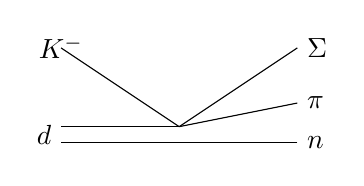
\begin{tikzpicture}
          \draw (-1.5,    1) node {$K^-$}--(0,    0);
          \draw (-1.5,    0)--(0,    0);
          \draw (-1.5, -0.2)--(0, -0.2);
          
          \node (d) at (-1.5, -0.1) [left] {$d$};
          
          \draw ( 1.5,  1.0) node [right] {$\Sigma$} -- (0,    0);
          \draw ( 1.5,  0.3) node [right] {$\pi$}    -- (0,    0);
          \draw ( 1.5, -0.2) node [right] {$n$}      -- (0, -0.2);
        \end{tikzpicture}
        \\
        (a) 1-step reaction
          
        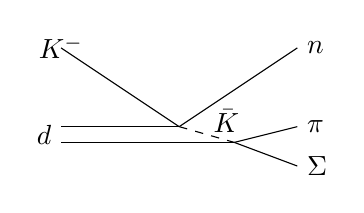
\begin{tikzpicture}
          \draw (-1.5,    1) node {$K^-$}--(0,    0);
          \draw (-1.5,    0)--(0,    0);
          \draw (-1.5, -0.2)--(0.7, -0.2);
          \node (d) at (-1.5, -0.1) [left] {$d$};
          
          \draw (0, 0) -- (0.7, -0.2) [dashed];
          \node (barK) at (0.6, -0.2) [above] {$\bar{K}$};
          
          \draw ( 1.5,  -0.5) node [right] {$\Sigma$} -- (0.7, -0.2);
          \draw ( 1.5,  -0.0) node [right] {$\pi$}    -- (0.7, -0.2);
          \draw ( 1.5,  1.0) node [right] {$n$}      -- (0,    0);
        \end{tikzpicture}
        \\
        (b) 2-step reaction
      \end{figure}
    \end{minipage}
  \end{tabular}
\end{frame}
